\documentclass{article}
\PassOptionsToPackage{numbers,sort&compress}{natbib}
\usepackage[preprint]{neurips_2026}
\usepackage[utf8]{inputenc}
\usepackage[T1]{fontenc}
\usepackage{graphicx}
\usepackage{booktabs}
\usepackage{amsmath}
\usepackage{microtype}
\usepackage[hidelinks]{hyperref}
\usepackage{url}
\usepackage{float}
\graphicspath{{figures/}}
\hypersetup{pdftitle={Denoising Diffusion for Histopathology Images},pdfauthor={Cai Xinyan}}

\title{Denoising Diffusion for Histopathology Images}
\author{Cai Xinyan\\ECE 285: Deep Generative Models, University of California, San Diego}
\date{}

\begin{document}
\maketitle

\begin{abstract}
We train an unconditional DDPM on 5,179 RGB histopathology images from the assigned Kaggle dataset. A 128$\times$128 U-Net uses a cosine schedule, EMA, and RGB covariance whitening estimated from 128 training images. We select the epoch-25 EMA checkpoint using a fixed-seed color diagnostic. On 5,000 generated and 5,000 training images, it obtains an Inception Score (IS) of 2.335 and an Ignite FID of 0.0618. Since the real reference is not held out, these scores are descriptive.
\end{abstract}

\section{Data and method}
We use the Histopathology subset of version 1 of the assigned Scientific Image Classification Dataset \citep{datafinal}, containing 5,179 RGB images. Images are center-fitted to $128\times128$, mapped to $[-1,1]$, and augmented with random flips and right-angle rotations.

A time-conditioned U-Net predicts the noise added under the DDPM objective \citep{ho2020ddpm}, with a cosine schedule ($T=1000$), AdamW, and EMA. We whiten RGB channels using their mean and covariance from 128 training images, then invert this transform for sampling. We generate images with 50-step DDIM \citep{song2021ddim}.

\begin{table}[H]
\centering
\small
\caption{Training and sampling settings.}
\label{tab:settings}
\begin{tabular}{ll}
\toprule
Setting & Value \\
\midrule
Images / resolution / U-Net & 5,179 / $128\times128$ RGB / 64 channels \\
Batch size / epochs & 32 / 100 \\
Optimizer & AdamW, learning rate $2\times10^{-4}$ \\
Schedule / objective & Cosine, 1,000 steps / noise MSE \\
EMA decay / color & 0.999 / RGB whitening, clip $\pm1.5$ \\
Sampling / hardware & DDIM, 50 steps / RTX 3090 \\
Seed & 43 \\
\bottomrule
\end{tabular}
\end{table}

\section{Results}
Training loss decreases from 0.536 at epoch 1 to 0.0696 at epoch 25 and 0.0608 at epoch 100. We select epoch 25: among the compared checkpoints, it has the closest fixed-seed RGB mean to a 128-image training reference and the least clipping. This diagnostic is only a selection aid, not independent validation.

Figure~\ref{fig:results} shows the loss history and sixteen selected-checkpoint samples. They capture varied stain colors and tissue-like textures, but remain smooth and sometimes blotchy, with limited fine cellular detail.

We compare 5,000 generated images with a deterministic 5,000-image subset of the training collection using PyTorch-Ignite's IS and default FID \citep{ignite}. This is not a held-out test. Ignite's FID uses 1,000-dimensional Inception logits, so it is implementation-specific and not directly comparable with the common 2,048-dimensional pool-feature FID.

\begin{table}[H]
\centering
\small
\caption{Epoch-25 EMA evaluation.}
\label{tab:metrics}
\begin{tabular}{lr}
\toprule
Metric & Result \\
\midrule
Inception Score (5,000 generated images) & 2.335 \\
FID (5,000 generated / 5,000 real) & 0.0618 \\
DDIM steps & 50 \\
\bottomrule
\end{tabular}
\end{table}

\begin{figure}[H]
\centering
\begin{minipage}[t]{0.41\linewidth}
\vspace{0pt}\centering
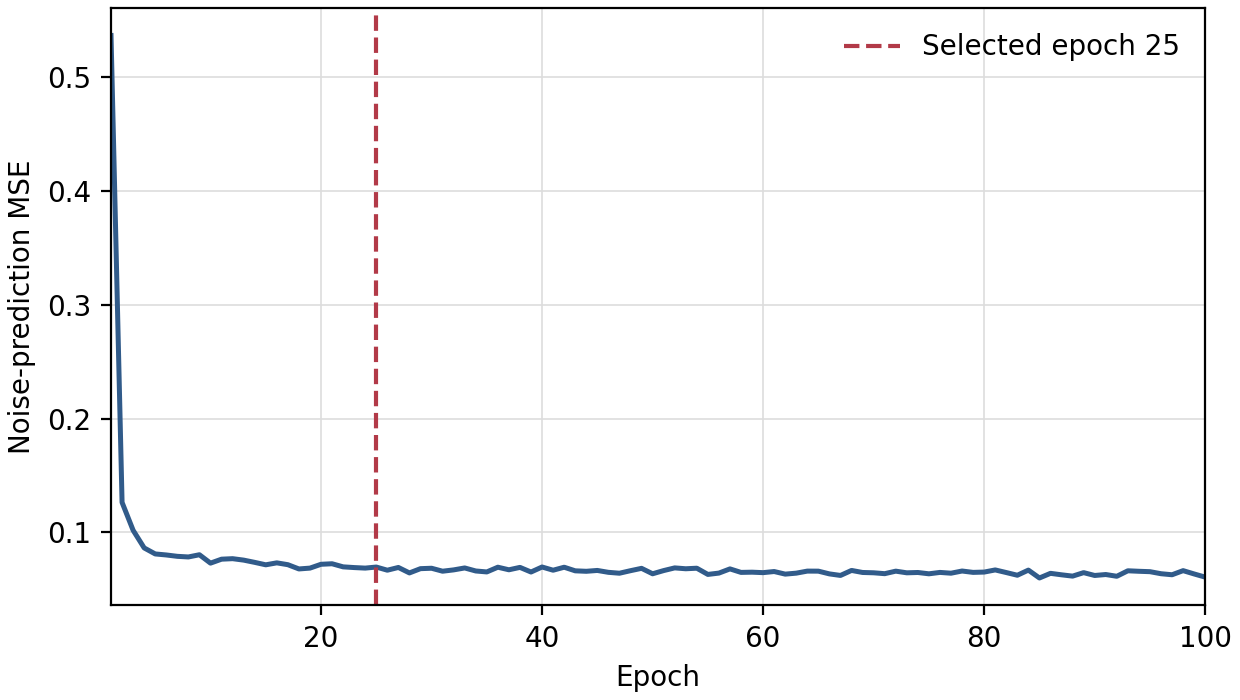
\includegraphics[width=\linewidth]{loss_curve_epoch25.png}
\end{minipage}\hfill
\begin{minipage}[t]{0.41\linewidth}
\vspace{0pt}\centering
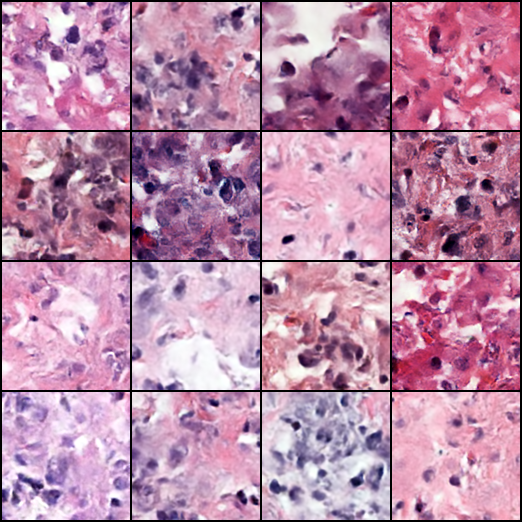
\includegraphics[width=\linewidth]{generated_epoch25.png}
\end{minipage}
\caption{Left: noise-prediction training loss across 100 epochs; the dashed line marks the selected epoch 25. Right: sixteen samples from its EMA checkpoint.}
\label{fig:results}
\end{figure}

\section{Discussion}
The model learns stain and texture patterns but not realistic fine morphology. Checkpoint selection uses a limited color diagnostic, and evaluation on training images cannot establish generalization. Report, code, and results:  \url{https://github.com/Serina-cinna/ece285-hw3}.

\small
\bibliographystyle{plainnat}
\bibliography{references}
\end{document}
